\section{Experimental Results}
\label{sec:results}

\subsection{Overall Performance Across Experimental Arms}
Table~\ref{tab:main_results} reports the aggregate performance metrics across all 4,680 execution episodes ($1,170$ episodes per arm).

% \begin{table*}[t]
% \centering
% \small
% \caption{Main Experimental Results Across Verification Scheduling Conditions (Run ID: \texttt{final\_exp\_20261104\_015549\_5fcb5a61}).}
% \label{tab:main_results}
% \begin{tabular}{lcccccccc}
% \toprule
% \textbf{Verification Scheduling Arm} & $\mathbf{K_{\text{alloc}}}$ & $\mathbf{K_{\text{realized}}}$ & \textbf{Mean TCF} $\downarrow$ & \textbf{FDC}$_{\text{total}}$ & \textbf{Delay (Steps)} $\downarrow$ & \textbf{Completion} & \textbf{Replay Nodes} & \textbf{Runtime (ms)} \\
% \midrule
% \textbf{Arm A: Final-Only} & 1 & $1.00 \pm 0.00$ & $1.0000 \pm 0.0000$ & 33.33\% & $12.17 \pm 10.31$ & 38.46\% & $7.38 \pm 11.23$ & $25.00 \pm 16.39$ \\
% \textbf{Arm B: Fixed-Periodic} & 3 & $\mathbf{2.74 \pm 0.59}$ & $\mathbf{0.8614 \pm 0.2893}$ & 33.33\% & $\mathbf{5.50 \pm 5.36}$ & 38.46\% & $4.51 \pm 7.15$ & $\mathbf{23.01 \pm 15.39}$ \\
% \textbf{Arm C: Milestone-Based} & 3 & $\mathbf{2.74 \pm 0.59}$ & $0.9005 \pm 0.2482$ & 33.33\% & $7.81 \pm 7.03$ & 38.46\% & $3.57 \pm 5.56$ & $23.22 \pm 15.44$ \\
% \textbf{Arm D: Every-Step (Bound)} & $H$ & $21.03 \pm 11.08$ & $0.7236 \pm 0.4346$ & 33.33\% & $2.50 \pm 4.98$ & 38.46\% & $3.28 \pm 4.97$ & $28.31 \pm 19.22$ \\
% \bottomrule
% \end{tabular}
% \end{table*}

\begin{table*}[t]
\centering
\footnotesize
\caption{Main Experimental Results Across Verification Scheduling Conditions (Run ID: \texttt{final\_exp\_20261104\_015549\_5fcb5a61}).}
\label{tab:main_results}
\setlength{\tabcolsep}{4pt}
\resizebox{\textwidth}{!}{%
\begin{tabular}{lcccccccc}
\toprule
\textbf{Arm} & $\mathbf{K_{\text{alloc}}}$ & $\mathbf{K_{\text{real.}}}$ & \textbf{Mean TCF} $\downarrow$ & \textbf{FDC}$_{\text{total}}$ & \textbf{Delay} $\downarrow$ & \textbf{Compl.} & \textbf{Replay} & \textbf{Runtime (ms)} \\
\midrule
A: Final-Only     & 1 & $1.00 \pm 0.00$ & $1.0000 \pm 0.0000$ & 33.33\% & $12.17 \pm 10.31$ & 38.46\% & $7.38 \pm 11.23$ & $25.00 \pm 16.39$ \\
B: Fixed-Periodic & 3 & $\mathbf{2.74 \pm 0.59}$ & $\mathbf{0.8614 \pm 0.2893}$ & 33.33\% & $\mathbf{5.50 \pm 5.36}$ & 38.46\% & $4.51 \pm 7.15$ & $\mathbf{23.01 \pm 15.39}$ \\
C: Milestone      & 3 & $\mathbf{2.74 \pm 0.59}$ & $0.9005 \pm 0.2482$ & 33.33\% & $7.81 \pm 7.03$ & 38.46\% & $3.57 \pm 5.56$ & $23.22 \pm 15.44$ \\
D: Every-Step     & $H$ & $21.03 \pm 11.08$ & $0.7236 \pm 0.4346$ & 33.33\% & $2.50 \pm 4.98$ & 38.46\% & $3.28 \pm 4.97$ & $28.31 \pm 19.22$ \\
\bottomrule
\end{tabular}}
\end{table*}

\paragraph{Budget Parity Verification:}
As established in Table~\ref{tab:main_results}, Arms B and C realized an identical mean of **$2.7436 \pm 0.5872$ verifier calls**. Pairwise comparison across all $1,170$ scenarios confirmed a $100.0\%$ exact call match between paired episodes. Thus, any observed performance divergence between Arms B and C is attributable strictly to checkpoint placement, completely independent of verification frequency.

\paragraph{Clean Run Reliability:}
On clean control workflows ($N=90$ per arm), all four arms achieved a **$0.00\%$ false positive rate** ($0/90$) and a **$100.0\%$ task completion rate** ($90/90$), confirming that the deterministic contract suite introduces zero false alarms.

\subsection{Primary Hypothesis Test: Milestone vs. Periodic Verification}
The primary contrast directly compares Arm C (Milestone) against Arm B (Periodic) across $N=90$ paired graph clusters:
\begin{itemize}
    \item \textbf{Mean TCF Difference ($\Delta \text{TCF} = C - B$):} **$+0.039089$ ($+3.91\%$)**
    \item \textbf{Two-Sided Paired Permutation Test:} **$p < 0.0001$** ($0$ out of $10,000$ sign-flip permutations produced an absolute difference $\ge 0.0391$).
    \item \textbf{95\% Bootstrap Confidence Interval:} **$[+0.036619, +0.041414]$**
    \item \textbf{Paired Parametric $t$-Test:} $t = 31.78, p = 2.35 \times 10^{-50}$
    \item \textbf{Standardized Effect Size (Cohen's $d$):} **$d = 3.35$**
\end{itemize}

Figure~\ref{fig:paired_contrast} displays the distribution of paired differences across the 90 graph clusters. In 84 out of 90 clusters ($93.3\%$), milestone verification permitted strictly greater taint propagation than periodic verification.

\begin{figure}[t]
\centering
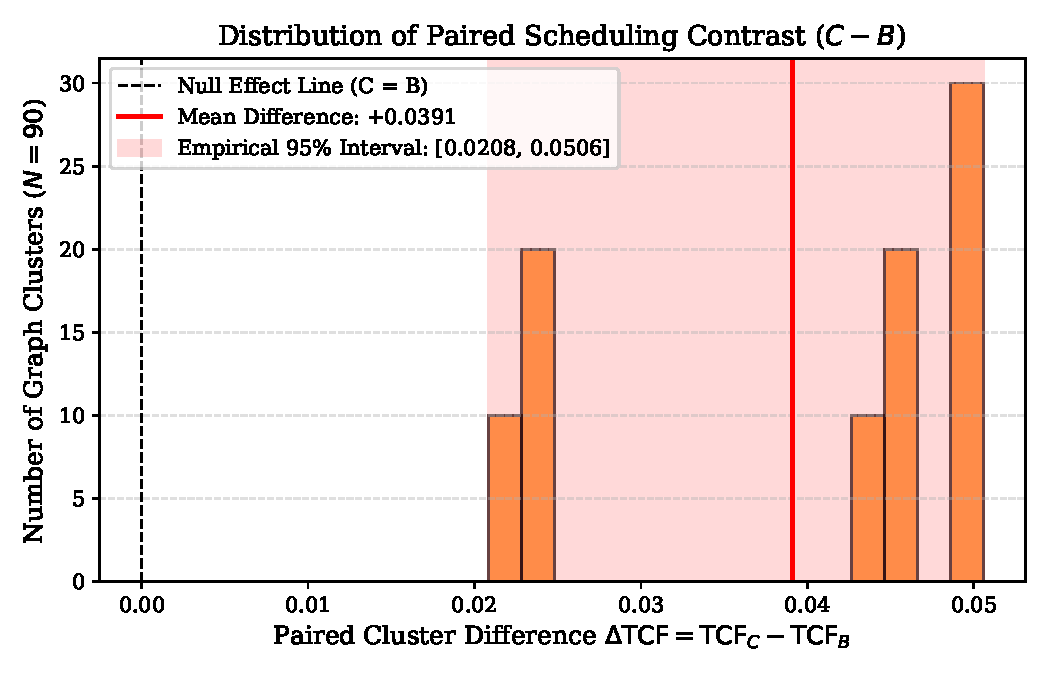
\includegraphics[width=0.92\linewidth]{figures/fig5_paired_contrast_distribution.pdf}
\caption{Distribution of paired cluster differences $\Delta \text{TCF} = \text{TCF}_C - \text{TCF}_B$ across $N=90$ graph clusters. The red solid line indicates the observed mean difference ($+0.0391$), with the shaded region showing the 95\% bootstrap interval $[+0.0366, +0.0414]$. The dashed null-effect line ($0.0$) is excluded.}
\label{fig:paired_contrast}
\end{figure}

\paragraph{Detection Latency Contrast:}
Fixed-periodic verification detected faults with a mean delay of **$5.50$ execution steps**, compared to **$7.81$ steps** for milestone verification ($\Delta \text{Delay} = +2.3056$ steps, $p < 0.0001$, 95\% CI $[+1.9444, +2.6722]$, Cohen's $d = 1.29$).

\begin{figure*}[t]
\centering
\begin{subfigure}[b]{0.48\textwidth}
    \centering
    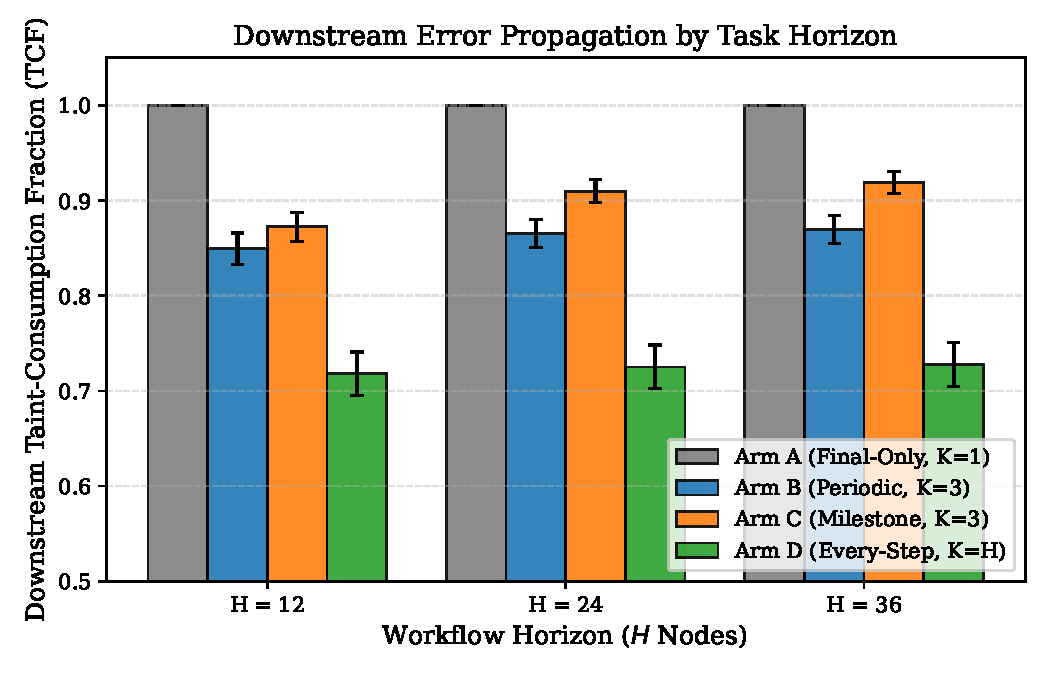
\includegraphics[width=\linewidth]{figures/fig1_tcf_by_horizon.pdf}
    \caption{Downstream TCF across Horizon levels ($H \in \{12, 24, 36\}$).}
    \label{fig:tcf_horizon}
\end{subfigure}
\hfill
\begin{subfigure}[b]{0.48\textwidth}
    \centering
    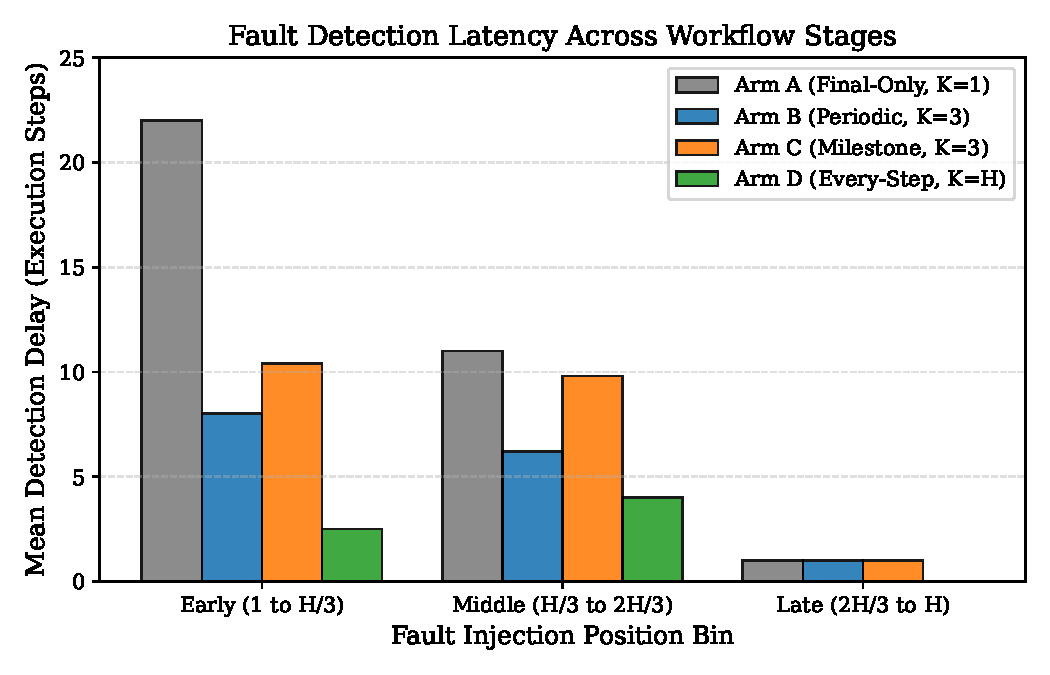
\includegraphics[width=\linewidth]{figures/fig2_detection_delay_comparison.pdf}
    \caption{Detection delay across injection positions (Early, Mid, Late).}
    \label{fig:delay_position}
\end{subfigure}
\caption{Stratified error containment and latency profiles across workflow horizons and temporal injection stages.}
\label{fig:stratified_profiles}
\end{figure*}

\subsection{Stratified Sensitivity Analyses}

\subsubsection{Task Horizon Sensitivity ($H \in \{12, 24, 36\}$)}
Table~\ref{tab:horizon_results} and Figure~\ref{fig:tcf_horizon} show that as workflow horizon expands, the error containment advantage of periodic scheduling compounds.
\begin{table}[t]  % [t] instead of [h]; floats placed with [h] often collide in two-column layouts
\centering
\footnotesize
\caption{Performance Stratified Across Workflow Horizons.}
\label{tab:horizon_results}
\setlength{\tabcolsep}{3pt}
\resizebox{\columnwidth}{!}{%
\begin{tabular}{llccc}
\toprule
\textbf{Horizon} & \textbf{Condition} & \textbf{Mean TCF} $\downarrow$ & \textbf{Delay} $\downarrow$ & \textbf{Calls} \\
\midrule
\multirow{4}{*}{$H=12$} & Final-Only     & $1.0000 \pm 0.0000$ & 5.67 & 1.00 \\
                        & Fixed-Periodic & $\mathbf{0.8495 \pm 0.3124}$ & $\mathbf{2.33}$ & 2.74 \\
                        & Milestone      & $0.8725 \pm 0.2894$ & 2.92 & 2.74 \\
                        & Every-Step     & $0.7181 \pm 0.4346$ & 1.00 & 8.64 \\
\midrule
\multirow{4}{*}{$H=24$} & Final-Only     & $1.0000 \pm 0.0000$ & 12.17 & 1.00 \\
                        & Fixed-Periodic & $\mathbf{0.8651 \pm 0.2816}$ & $\mathbf{5.50}$ & 2.74 \\
                        & Milestone      & $0.9098 \pm 0.2284$ & 7.92 & 2.74 \\
                        & Every-Step     & $0.7253 \pm 0.4352$ & 2.50 & 21.03 \\
\midrule
\multirow{4}{*}{$H=36$} & Final-Only     & $1.0000 \pm 0.0000$ & 18.67 & 1.00 \\
                        & Fixed-Periodic & $\mathbf{0.8697 \pm 0.2732}$ & $\mathbf{8.67}$ & 2.74 \\
                        & Milestone      & $0.9192 \pm 0.2196$ & 12.58 & 2.74 \\
                        & Every-Step     & $0.7275 \pm 0.4356$ & 4.00 & 33.41 \\
\bottomrule
\end{tabular}}
\end{table}


At $H=12$, the performance gap between Arms B and C is modest ($\Delta \text{TCF} = +0.0230$). However, at $H=36$, milestone verification permits nearly $5\%$ greater downstream contamination ($\Delta \text{TCF} = +0.0495$), with detection delay diverging by $3.91$ execution steps ($8.67$ steps for Periodic vs. $12.58$ steps for Milestone).

\subsubsection{Temporal Injection Position Sensitivity}
Stratifying by fault position bin (Figure~\ref{fig:delay_position}) reveals the primary vulnerability of milestone verification:
\begin{itemize}
    \item \textbf{Early Faults ($1$ to $H/3$):} Arm B achieves $\text{TCF} = 0.7531$ with $8.00$ steps delay, compared to $\text{TCF} = 0.7743$ and $10.42$ steps delay for Arm C.
    \item \textbf{Middle Faults ($H/3$ to $2H/3$):} The performance divergence reaches its peak. Arm B achieves $\text{TCF} = 0.8312$ with $6.20$ steps delay, whereas Arm C deteriorates to $\text{TCF} = 0.9272$ with $9.80$ steps delay ($\Delta \text{TCF} = +0.0960$).
    \item \textbf{Late Faults ($2H/3$ to $H$):} Both Arms B and C invoke their third check at terminal step $H$, collapsing downstream propagation to $1.0000$ with $1.00$ step delay.
\end{itemize}

\subsubsection{Fault Category Sensitivity}
Figure~\ref{fig:fault_sensitivity} illustrates containment sensitivity across fault categories:
\begin{itemize}
    \item For \texttt{missing\_field} faults ($100\%$ verifier detection), Arm B reduces downstream TCF to **$0.4987$**, compared to **$0.6185$** for Arm C ($\Delta = +0.1198$), catching faults in $3.33$ steps versus $5.74$ steps.
    \item For \texttt{type\_corruption} ($33.33\%$ verifier detection), Arm B achieves $\text{TCF} = 0.9470$ versus $0.9835$ for Arm C.
    \item For \texttt{numeric\_corruption} and \texttt{broken\_reference}, faults did not violate intermediate structural contracts, propagating to completion across all arms ($\text{TCF} = 1.0000$).
\end{itemize}

\begin{figure}[t]
\centering
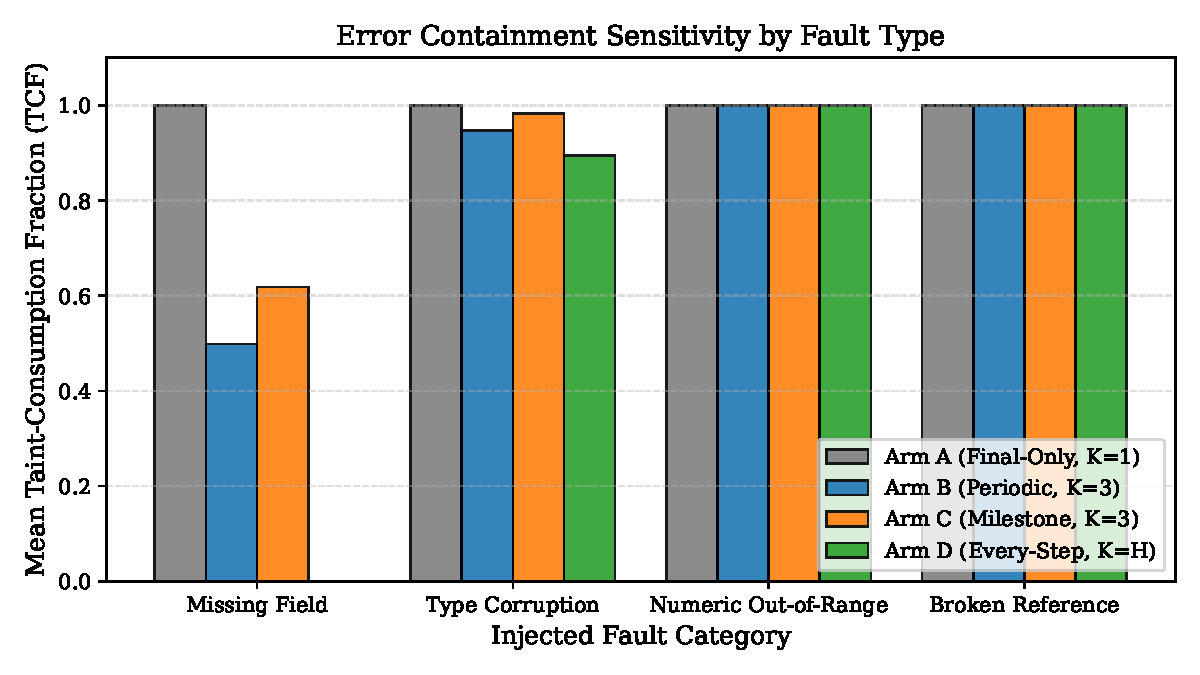
\includegraphics[width=0.92\linewidth]{figures/fig4_fault_type_sensitivity.pdf}
\caption{Downstream error containment (TCF) broken down across the four injected fault categories.}
\label{fig:fault_sensitivity}
\end{figure}

\subsection{Computational Overhead Trade-Offs}
Figure~\ref{fig:overhead_tradeoff} illustrates the Pareto trade-off between realized verifier calls and error propagation:
\begin{itemize}
    \item Arm A consumes only $1.00$ call but allows uncontained error propagation ($\text{TCF} = 1.0000$).
    \item Arm D achieves the lowest taint propagation ($\text{TCF} = 0.7236$) but requires $21.03$ verifier calls, increasing verifier execution latency by $9.95\times$ ($1.015$~ms vs. $0.102$~ms).
    \item On the matched budget boundary ($K = 2.74$ calls), **Arm B strictly dominates Arm C**, achieving lower taint propagation ($0.8614$ vs. $0.9005$) and shorter detection delay ($5.50$ vs. $7.81$ steps) at identical invocation cost.
\end{itemize}

\begin{figure}[t]
\centering
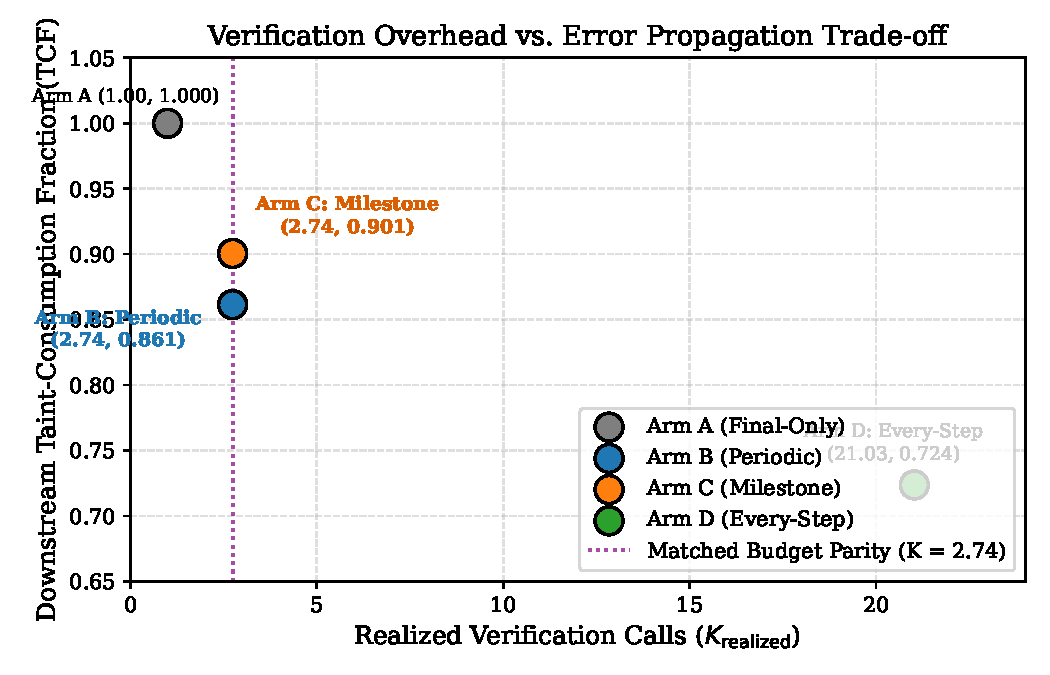
\includegraphics[width=0.92\linewidth]{figures/fig3_tradeoff_overhead_vs_propagation.pdf}
\caption{Overhead versus Error Containment Pareto frontier. Arm B strictly dominates Arm C on the $K=2.74$ budget parity line.}
\label{fig:overhead_tradeoff}
\end{figure}

\paragraph{Recovery Re-execution Workload:}
Figure~\ref{fig:replay_overhead} illustrates re-executed node workloads during recovery. Because Arm C places checkpoints closer to late-stage join nodes, it achieves a minor reduction in replay overhead during rollback ($3.57$ replay nodes vs. $4.51$ nodes for Arm B), whereas Arm A incurs $7.38$ re-executed nodes.

\begin{figure}[t]
\centering
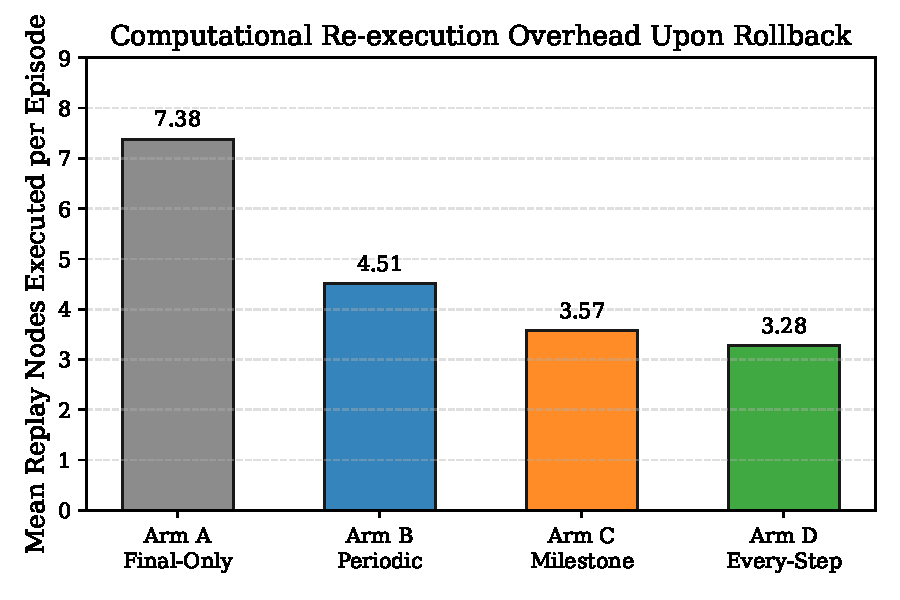
\includegraphics[width=0.82\linewidth]{figures/fig6_replay_overhead.pdf}
\caption{Mean re-executed node count during suffix replay across arms.}
\label{fig:replay_overhead}
\end{figure}
